%空行代表重启一个段落。
%开始插入附录
%\appendix
\chapter{附录J\quad 本研究中部分基因的核酸和蛋白序列}\label{appen:J}
%直接在奇数页页眉中显示章标题会多处一些章标题内部编号,这里重新定义\leftmark,后续所有章节都要重新定义
\renewcommand{\leftmark}{附录J\quad 本研究中部分基因的核酸和蛋白序列}
\noindent $>$The DNA and protein sequence of the Linker used in this study
\vspace{2mm}

%这里采用插入图片的方式对其序列。如果用xeLaTeX编译可以尝试TeXshade package。
\graphicspath{{figures/}}
%插入图片并设置图片宽度为文本宽度减10mm
\noindent 
\includegraphics[width=\textwidth-45mm]{figJ-3.jpg}

\noindent $>$The DNA sequence of \textit{yfp} used in this study
\vspace{2mm}

%这里采用插入图片的方式对其序列。如果用xeLaTeX编译可以尝试TeXshade package。
\graphicspath{{figures/}}
%插入图片并设置图片宽度为文本宽度减10mm
\noindent 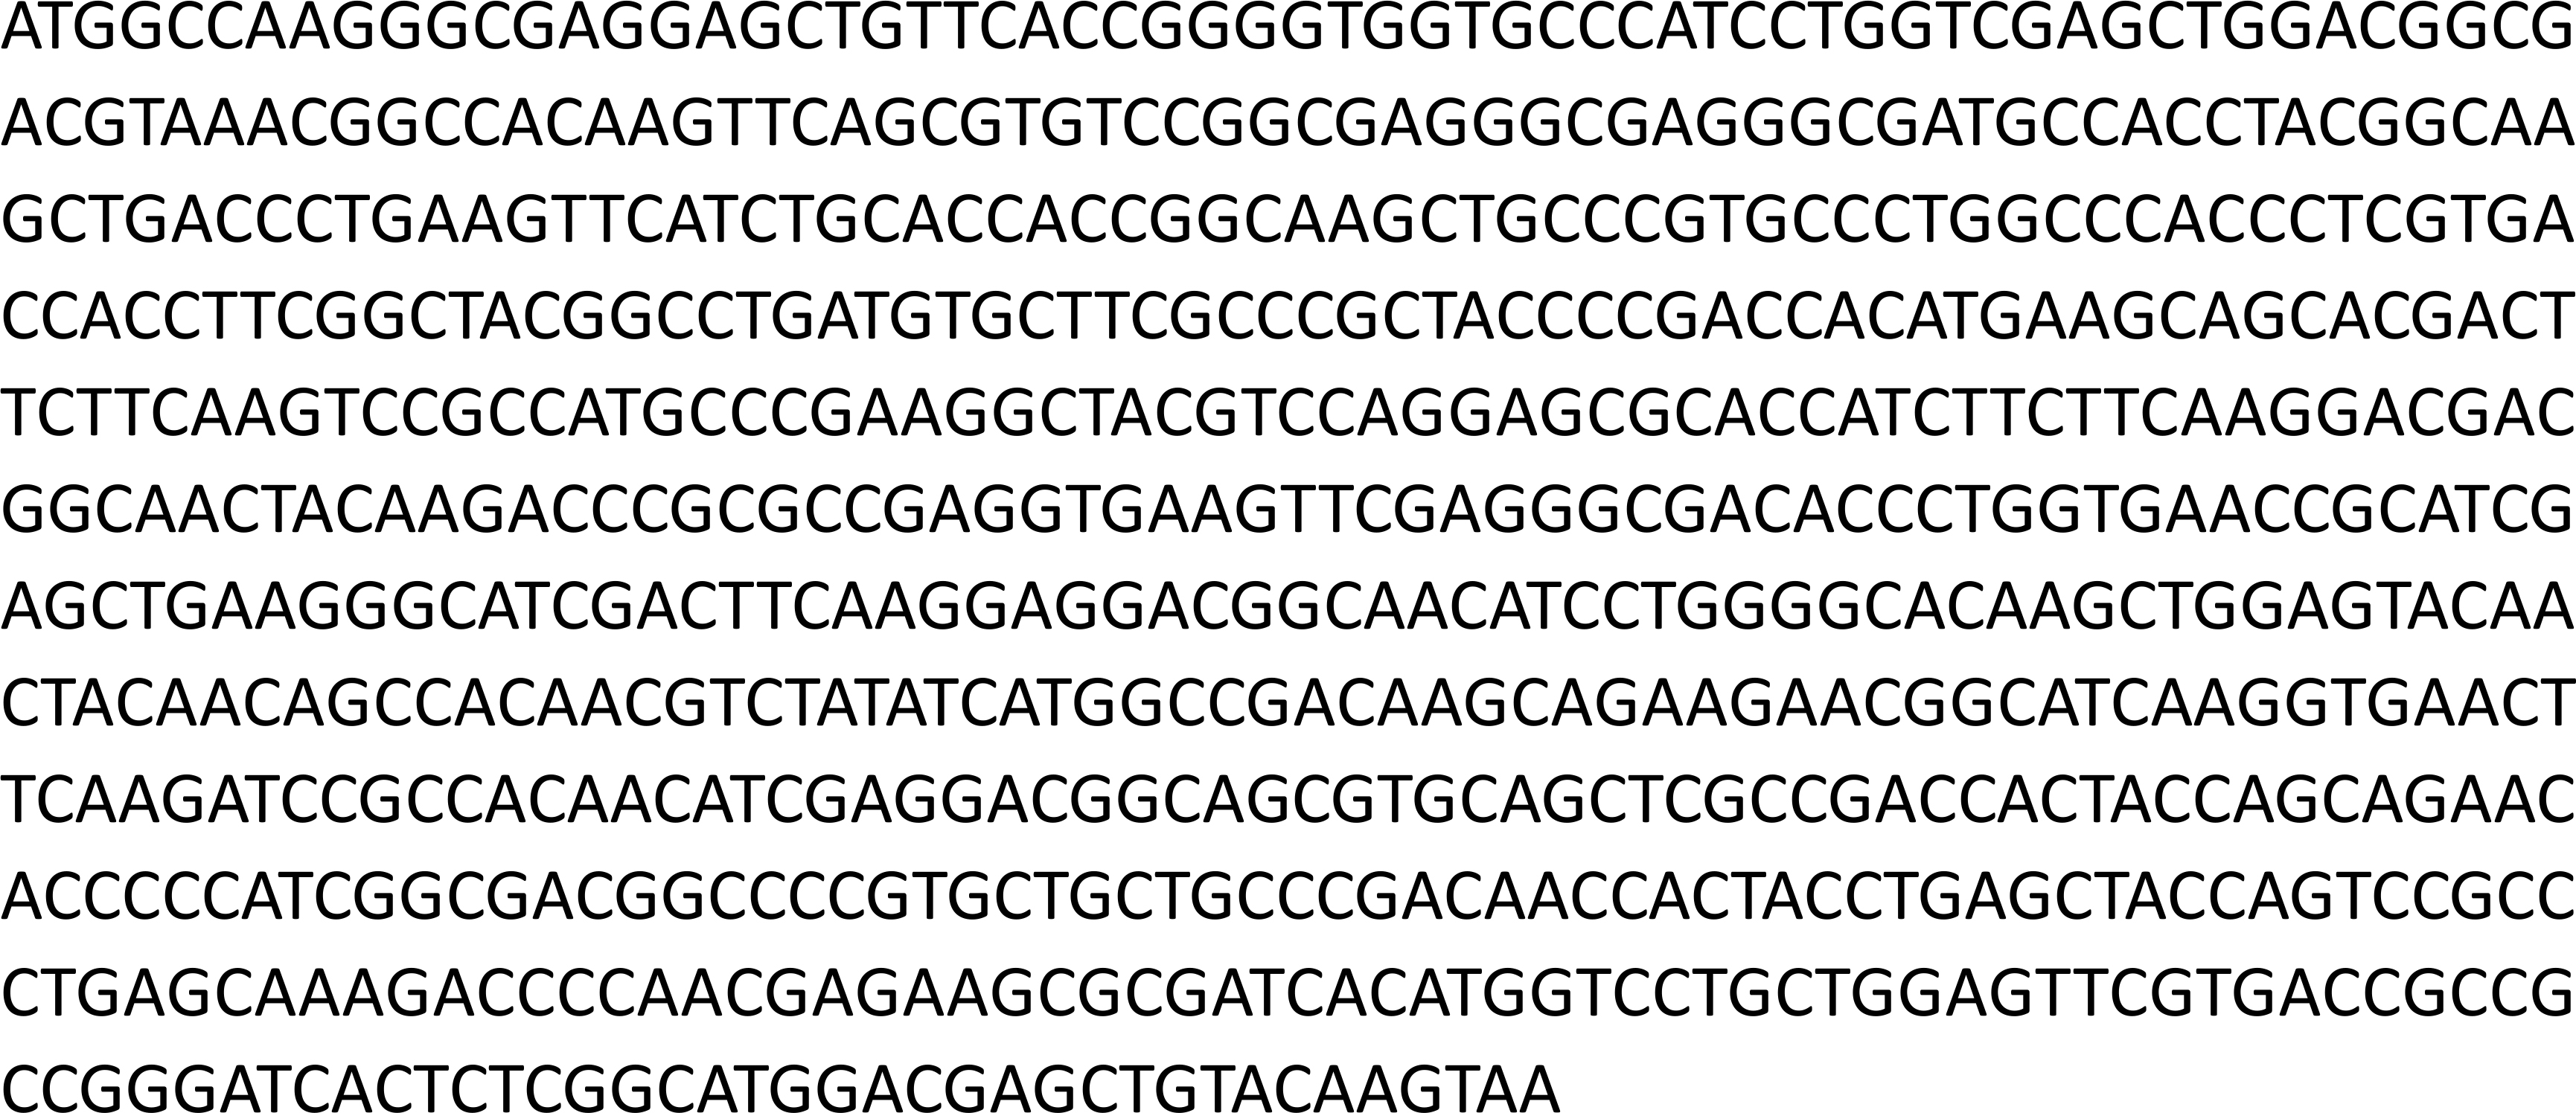
\includegraphics[width=\textwidth]{figJ-1.jpg}

\noindent $>$The protein sequence of YFP used in this study
\vspace{2mm}

\graphicspath{{figures/}}
%插入图片并设置图片宽度为文本宽度减10mm
\noindent 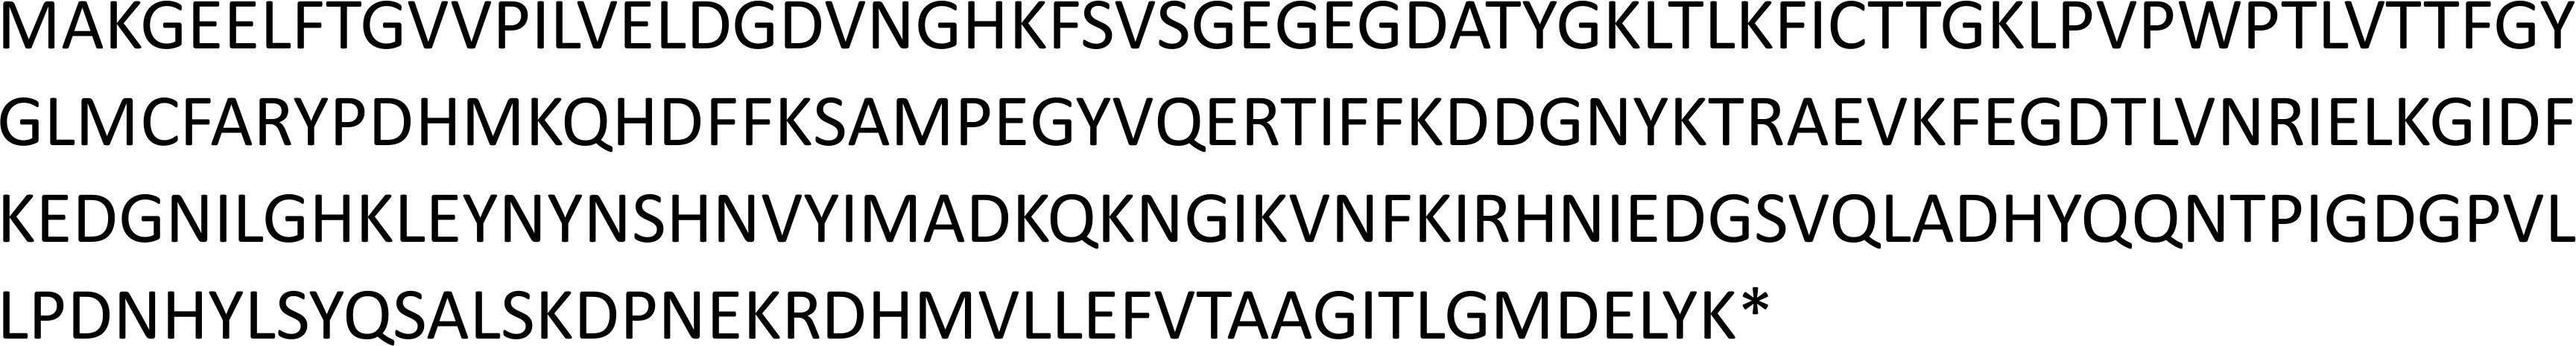
\includegraphics[width=\textwidth]{figJ-2.jpg}

\noindent $>$The DNA and protein sequence of the HA\footnote{Human influenza hemagglutinin} tag used in this study
\vspace{2mm}

%这里采用插入图片的方式对其序列。如果用xeLaTeX编译可以尝试TeXshade package。
\graphicspath{{figures/}}
%插入图片并设置图片宽度为文本宽度减10mm
\noindent 
\includegraphics[width=\textwidth-55mm]{figJ-4.jpg}

\noindent $>$The DNA and protein sequence of the SV40\footnote{Simian vacuolating virus 40} large T antigen NLS used in this study
\vspace{2mm}

%这里采用插入图片的方式对其序列。如果用xeLaTeX编译可以尝试TeXshade package。
\graphicspath{{figures/}}
%插入图片并设置图片宽度为文本宽度减10mm
\noindent 
\includegraphics[width=\textwidth-65mm]{figJ-5.jpg}
